\section{Introduction}

Humans actively use vision during everyday activities to gather and refine information about the environment. Since the seminal works of \citet{Yarbus2013-eu} and \citet{Buswell1935-di} there has been consistent evidence that eye movements depend on the viewing task the observer is performing. This is further supplemented by studies that have revealed that overt attention during natural viewing conditions is driven by scene semantics i.e. meaning and not by salience \citep{Henderson2017-it}. \citet{Kollmorgen2010-wg} have also shown that spatial viewing biases and task dependent features contribute highly to attention in a visual scene. We have growing evidence that eye movements are driven by top-down factors of task relevance and less by bottom-up factors of salience in the environment.

While studying eye movements profiles on static images in a controlled lab environment has offered illuminating insights into task-relevant modulation of attention, mobile subjects can give us a richer picture of cognitive processing in more naturalistic settings. In a pragmatic turn in cognitive science, there is a greater push towards incorporating the study of cognitive processes while interacting with the external world \citet{Parada2020-qq}. Moreover, \citet{Engel2013-bx} proposed that cognition encompasses the body and in turn, bodily action can be used to infer cognition. To this effect, understanding the control of eye movements in natural, real-life situations requires a mobile setup that allows for a subject to be recorded in tandem with volitional actions in a controlled yet unconstrained environment. In recent years, virtual reality (VR) and mobile sensing has offered great opportunity to create controlled, natural environments where subjects' eye and body movements can be measured reliably along with their interactions with the environment \citep{Keshava2020-cp, Clay2019-cu, Mann2019-ls}. Experiments in virtual environments have grown popular in recent years and have shown promise towards studying cognition in naturalistic and controlled environments.

Seminal studies have already investigated eye movement behavior in natural environment with fully mobile participants. For example, eye movements have been studied under a plethora of natural condition while walking \citep{Matthis2018-ho}, tea-making \citep{Land1999-ol} , sandwich making \citep{Hayhoe2003-lw} , driving \citep{Mars2012-bn, Sullivan2012-gg}, hand-washing \citep{Pelz2001-cn} , hitting a ball \citep{Land2000-pw}. For these studies head-mounted eye-tracking devices were used as participants performed these tasks that allowed for fully mobile interaction with the world. Although the head mounted camera and eye-tracker record the subjects' ego-centric view of the environment, there are still some deficiencies in precisely recording the changes in the environment simultaneously with bodily interactions in a unified space. Here, VR based studies can provide a unique solution to monitor time-resolved changes in the environment and the participant.

Experiments in naturalistic settings have revealed several distinct functions of the eye movements during everyday tasks. In the pioneering studies of \citet{Land1999-ol} and \citet{Hayhoe2003-lw}, subjects performed everyday activities of tea-making and sandwich-making, respectively. These studies required a sequence of actions which involved manipulating objects one at a time to achieve the goal. Both studies showed that nearly all the fixations were task-related. Furthermore, there was a systematic relative timing of visual fixation on object and manipulation where fixations were made to target objects about 600ms before manipulation. More importantly, \citet{Ballard1995-ji} proposed a \emph{"just-in-time"} strategy that universally applies to this relative timing of fixations and actions. In other words, they state that fixations that provide information for a particular action immediately precede that action and is crucial for a fast and economical execution of the task.

\citet{Land2001-do} posit that fixations can be broadly categorized into four functional groups; 'locating' fixations which retrieve visual information; 'directing' fixations which acquire the position information of an object and accompany a manipulation action and facilitate reaching movements; 'guiding' fixations which alternate between two objects being manipulated e.g. knife, bread, and butter; and 'checking' fixations which monitor where the task-constraints in the scene have been met. These findings have also been corroborated by \citet{Pelz2001-cn, Mennie2007-my}.

\citet{Pelz2001-cn} showed similar just-in-time strategy of gaze allocation while performing a hand-washing task. They also reported a small number of fixations \~5\% that did not serve the immediate sub-task but rather provided information that would be needed for a future action. The authors hypothesize these "look-ahead" fixations provide a mechanism to stabilize the visual input stream that result from a sequence of actions, facilitate task-switching, and reduce conscious effort required to complete the actions in a sequence. Hence, look-ahead fixations can be explained as a perceptual strategy to ease the cognitive load attending to complex tasks in the real world. In sum, the wide-ranging functions of eye movements are well documented in natural and routine tasks.

\citet{Land2001-do} also proposed a framework that outlines the flow of visual and motor control during task execution as shown in \textcolor{Blue}{Figure \ref{figure:task}A}. The process summarizes the various operations that \emph{must} occur during an 'object-related action' i.e., individual actions performed on separate objects to achieve the desired goal. As described in Land (2006) each schema " specifies the object to be dealt with, the action to be performed on it, and the monitoring required to establish that the action has been satisfactorily completed." Further, the gaze control samples the information about the location and identity of the object and directs the hands to it. Subsequently, the motor control system of the arms and hands implement the desired actions. Here, vision provides the information of where to direct the body, which state to monitor, and determine when the action must be terminated. Taken together, a 'script' of instructions is sequentially implemented where the eye movements earmark the task-relevant locations in the environment that demand attentional resources for that action.

% \begin{figure}[h]
%     \centering
%     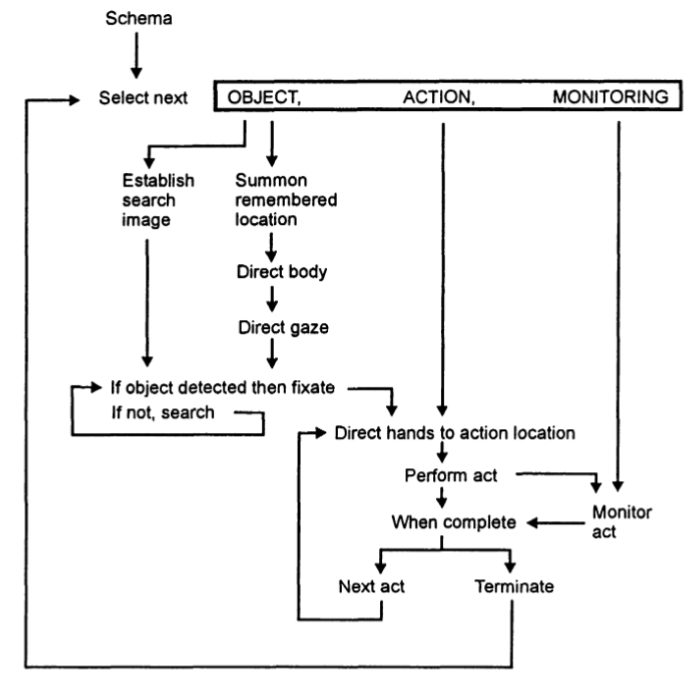
\includegraphics[width=0.6\linewidth]{source/figures/introduction/land_schema.PNG}
%     \caption{Schematic of motor and gaze control systems during performance of natural tasks. From \citet{Land2001-do}}
%     \label{fig:land_schema}
% \end{figure}

The common theme in the above studies is that the tasks investigated (tea-making, sandwich-making, hand-washing) have an organized task structure. These tasks involve specific object-related actions such as picking up the knife, picking up the teapot, etc. and have a predefined 'script' for the execution of the tasks. The studies, therefore, study eye movements that are under strict control of a task sequence. Moreover, these tasks are over-learned and over-generalized as they are part of a habitual action repertoire for an adult human being. As discussed by \citet{Land2006-da} these low level schemas defined above are likely not executed under deliberate conscious control. This distinction corresponds to \citet{james2007principles}'s distinction between "ideo-motor" and "willed" acts. As James described, ideo-motor actions correspond to movements where we are "aware of nothing between the conception and execution" of the said action. In contrast, the willed actions require "an additional conscious element in the shape of a fiat, mandate, or expressed consent." Hence, it is unclear whether these low-level schemas of gaze control operate similarly for deliberate actions where an internal task 'script' is not already known.

\citet{Norman1986-qb} proposed a theoretical framework for the components of attentional mechanisms that govern deliberate/planned actions. In comparison to the low-level schema proposed by Land \& Hayhoe which can account for routine, well-learned tasks, the \citet{Norman1986-qb} model suggests another supervisory module that selects a schema to implement. In well-learned tasks, a schema is triggered automatically without conscious control. However, when a task is fairly complex and requires planning, multiple low-level schemas might compete for resources at the same time and require \emph{contention scheduling}. For example, contentions can arise on whether to monitor the current action with respect to previous actions or future planned actions to fulfill the task-relevant goals. Such a scheduling mechanism is then required to provide conflict resolution for potentially relevant schemas either by inhibition or activation. Additionally, the model proposes a Supervisory Attentional System (SAS) that modulates the selection of a schema. The model suggests that attentional resources are deployed only at the specific points in a task where schema selection is required. Taken together, the model predicts that a failure of the supervisory control can lead to an instability of attention and heightened distraction.

In the present study, we investigate the mechanisms of allocation of attention while performing a novel task in a naturalistic environment. We created two types of tasks that varied in complexity and required performing a sequence of actions to accomplish the cued goal. We asked subjects to sort objects on a life-size shelf based on the object features. The complexity of the task depended on sorting based on one object feature or both. We designed the tasks to be novel in a way that subjects had to plan their action sequences on-the-fly and in absence of a pre-defined action "script". We concurrently measured the eye and body movements while subjects performed the tasks. 

% Based on the models proposed by \citet{Land2001-do} and \citet{Norman1986-qb}, we predicted four behavioral outcomes:
% \begin{enumerate}
%     \item if the actions are deliberately and optimally planned, subjects would exhibit targeted gaze guidance towards task-relevant objects. Conversely, eye movement would be more random showing more search behavior when actions are produced randomly and without deliberation.
%     \item optimal planning of action would require gaze allocation to target locations of previous actions to monitor task requirements are validated by current actions.
%     \item with optimal selection of relevant action schemas, subjects would allocate gaze to task-locations relevant to the actions in the future action sequence.
%     \item given optimal gaze allocation towards current task-relevant locations would not be just-in-time i.e. first fixations on the target objects would not immediately precede an action. 
% \end{enumerate}

% Overall, these predictions generalize the flow of low-level schemas proposed by \citet{Land2001-do} by taking into account a novel task which forces deliberate action planning.



